\subsection{Online Clustering}
\label{subsec:5b_online_clustering}

\subsubsection{Setup}
\label{subsubsec:5b_setup}

The online clustering is done on a simulated stream of news articles
based on the same data set as used in the clustering evaluation.
This allows for direct comparison between the detected events and the ground truth.
The settings to run the clustering are as follows:

\begin{itemize}
    \item Preprocessing: Text Lemmatization
    \item Vector space model: tf-idf
    \item Clustering method: HDBSCAN
    \item Minimum cluster size: 6
    \item Metric: cosine
\end{itemize}

The clustering is run over 30 days with a total of 42,916 news articles.
The distribution of news articles during this time period is illustrated in \figref{fig:news_articles_over_time}.
The time delta, which is the amount of time between two batches, is set to one hour.

\begin{figure}[h]
    \centering
    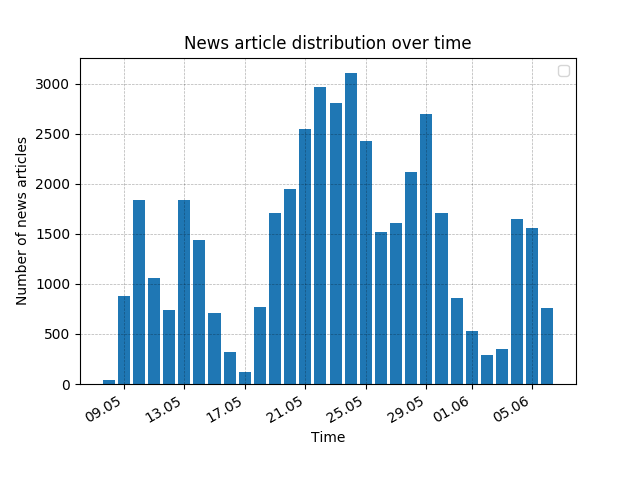
\includegraphics[width=0.5\textwidth]{news_articles_over_time}
    \caption{Incoming news articles over 30 days.}
    \label{fig:news_articles_over_time}
\end{figure}

\subsubsection{Evaluation}
\label{subsubsec:5b_evaluation}

The goal of the online clustering is to detect new events in an incoming stream
of news articles and changes in existing events.

\paragraph{Static batch sizes}
We start the evaluation with static batch sizes.
\figref{fig:event_detection_differences} shows the differences between the number of detected events
and the number of true events for both new and existing topics.
Based on this data we see the impact of different batch sizes for the precision in detected events.
The difference with a batch size of 5,000 news articles is considerably lower than with a batch size of 1,000.
The difference is especially noticeable in the time period between the 21.05 and 25.05.
The reason for this spike can be found in the distribution of incoming news articles
as shown in \figref{fig:news_articles_over_time}.
During this period we receive up to 3,000 news articles in a single day.
This means by using a lower batch size such as 1,000,
the overlap between batches gets too small to reliably detect changes between batches,
which causes too many new topics to be detected.

\begin{figure}[h]
    \centering
    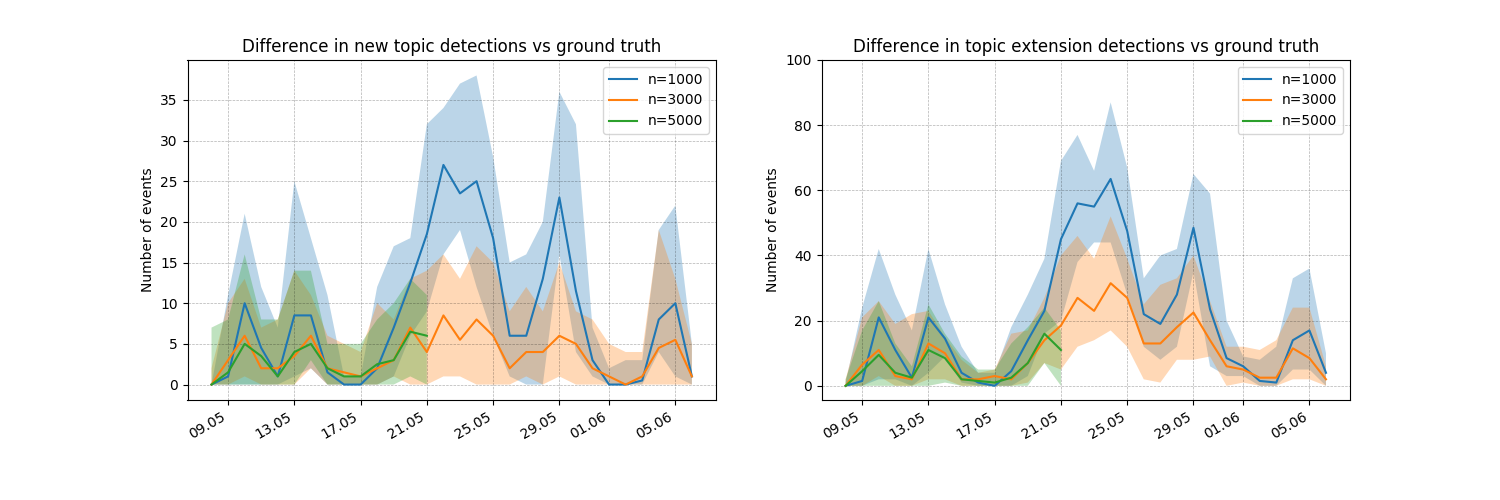
\includegraphics[width=1\textwidth]{event_detection_differences}
    \caption{
        Comparison between the difference in detected and true events.
        The line represents the median, while the area shows the range from the minimum to the maximum value.
    }
    \label{fig:event_detection_differences}
\end{figure}

Although a larger batch size does not simply equal a better difference,
as can be seen in \figref{fig:event_detection_differences}
by comparing the differences using a batch size of 3,000 with a batch size of 5,000.
The batch size n=3000 shows a generally lower difference in the detection of new events than with n=5000.
The differences between both batch sizes are smaller when detecting changes in existing events.

Based on the overall differences, we do not know the precision of those predictions.
If the difference between newly detected events and true events is zero,
there is still the possibility, that the events are different from the ground truth,
and thus contain false positives.
To measure the quality of events, we can look at the collection of events in a single batch as a subset of clusters,
where each event is represented by a cluster containing all relevant news articles.
Since we now have two clusterings, one containing detected events and the other with events taken from the ground truth,
we can apply our MP-Score as a metric to get an insight into the precision of the detected events.
\figref{fig:event_detection_mp_score_1000} shows the MP-Scores for an online clustering using a batch size of 1,000.
Since there is quite a large variance, the score is shown as a boxplot, where a single box represents a full day.
The large variance is already the first indication, that the quality is rather low.
Meaning that there are still many false positives and false negatives.

\begin{figure}[h]
    \centering
    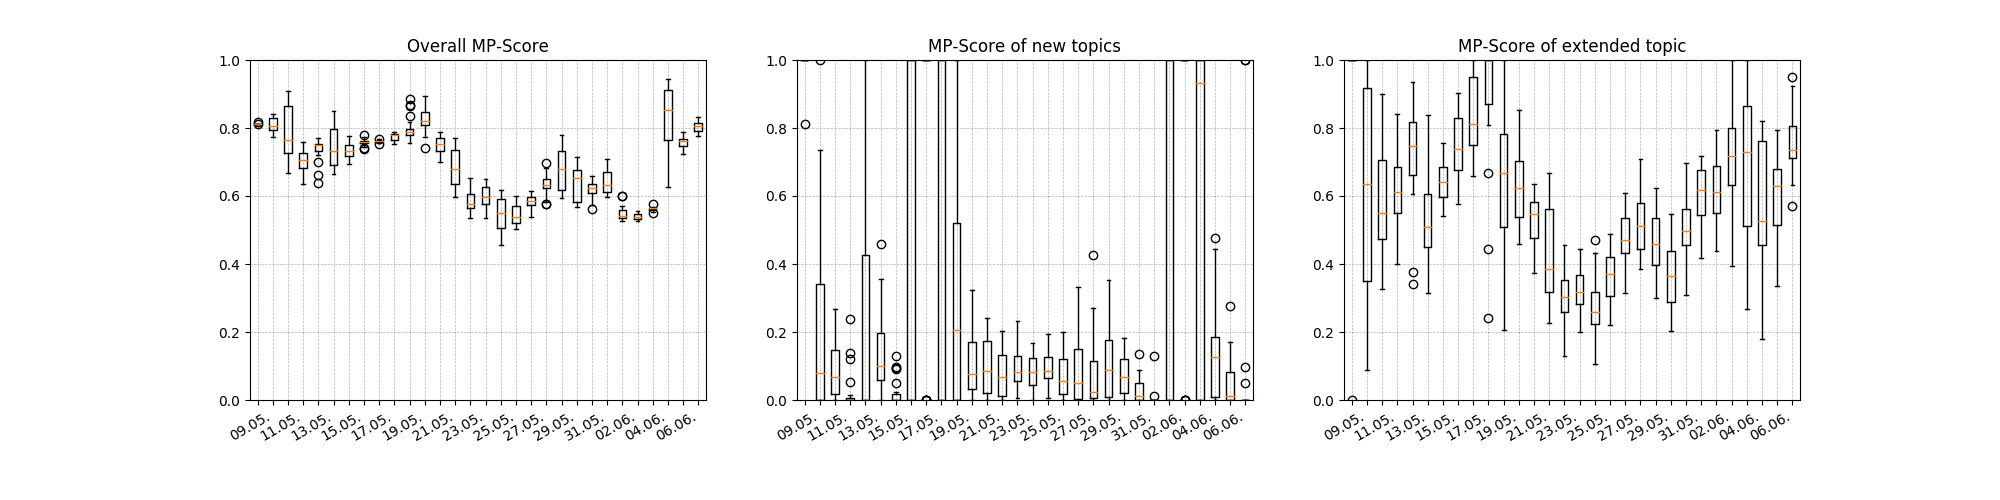
\includegraphics[width=1\textwidth]{event_detection_mp_score_1000}
    \caption{MP-Scores for clusterings using batch size of 1000.}
    \label{fig:event_detection_mp_score_1000}
\end{figure}

Looking at an increased batch size of 5,000 in \figref{fig:event_detection_mp_score_5000},
we note that there is less variance in the overall score, which compares the full clustering with the ground truth.
Although the variance for new and existing event detections is still fairly high.
Additionally while the variance is high, the median for new topics is mostly around 0.1.
This tells us that most of the newly detected events do not correspond with new events according to the ground truth.
The detection of extensions of existing events is generally more accurate
with a median between 0.5 and 0.8 using n=5000, but there is still are wide variance noticeable.

\begin{figure}[h]
    \centering
    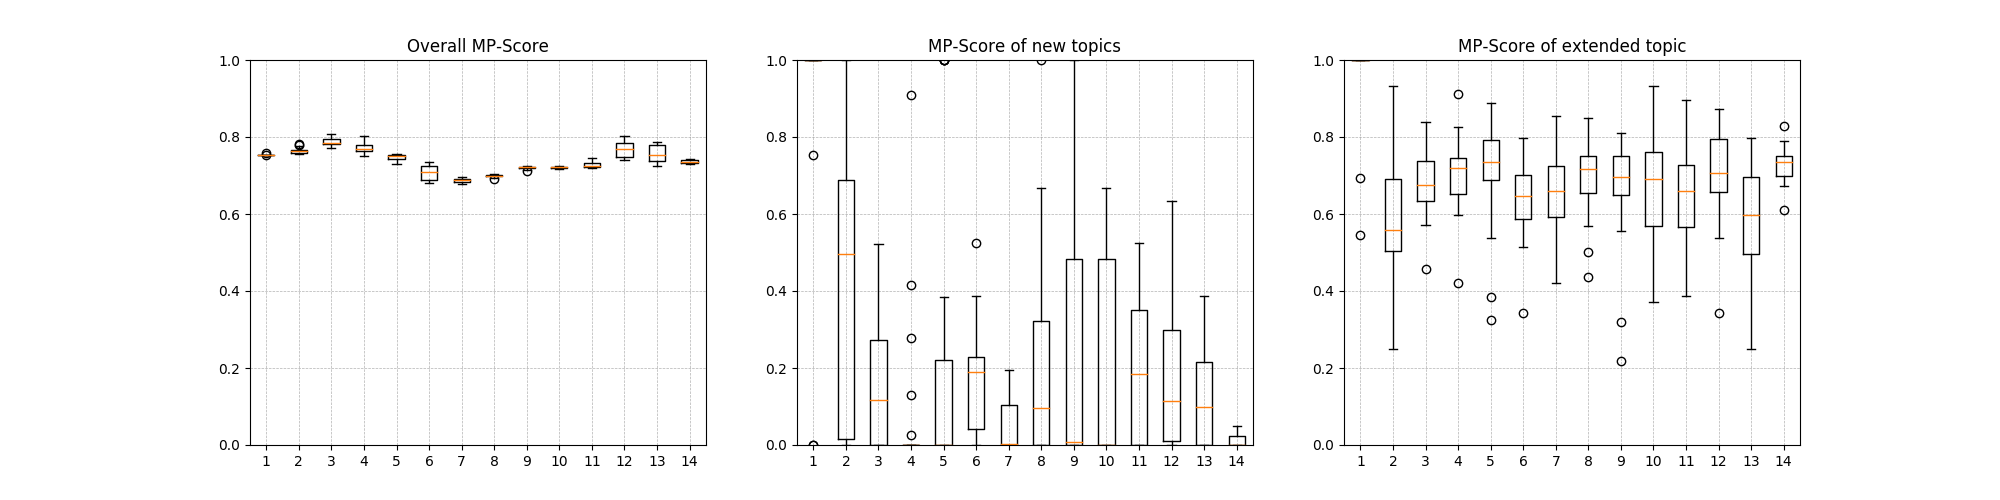
\includegraphics[width=1\textwidth]{event_detection_mp_score_5000}
    \caption{MP-Scores for clusterings using batch size of 5000.}
    \label{fig:event_detection_mp_score_5000}
\end{figure}

One of the reasons for the difference in the precision of the detection of new events and the extension of events
might be explained by the minimum cluster size.
In the current setting the minimum cluster size is set to 5,
which means if a new event occurs containing only four news articles,
it will be discarded as noise.
If the second batch contains additional news articles for the same event,
it will be detected as a new occurrence, but the ground truth treats it as an existing event. 
This increases the difference between detections and the ground truth.
To see how this affects the result we run the same simulation with a batch size of n=3000 a second time,
but only considering new events from the ground truth
if the number of news articles is greater or equal to the minimum cluster size.

\begin{figure}[h]
    \centering
    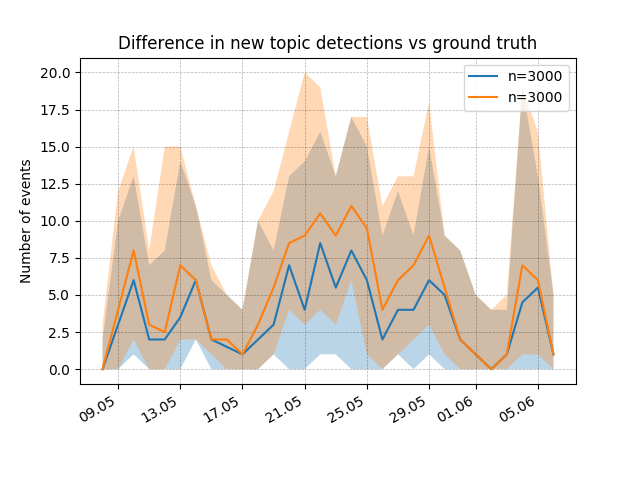
\includegraphics[width=0.5\textwidth]{event_detection_differences_with_min_cluster_size}
    \caption{Differences in predictions vs ground truth using batch size of 3000.}
    \label{fig:event_detection_differences_with_min_cluster_size}
\end{figure}

Limiting new events in the ground truth based on the minimum cluster size
gives the opposite result as initially expected.
\figref{fig:event_detection_differences_with_min_cluster_size} clearly shows
an increase in the difference between predicted events and the adjusted ground truth.
This means we already detected more new events than there were present in the ground truth
and limiting it based on the minimum cluster size only lowered the true number of events,
thus leading to an increase in the difference.
A look at the raw data from an initial simulation run in \figref{fig:event_detection_by_date_3000}
validates this assumption.

\begin{figure}[h]
    \centering
    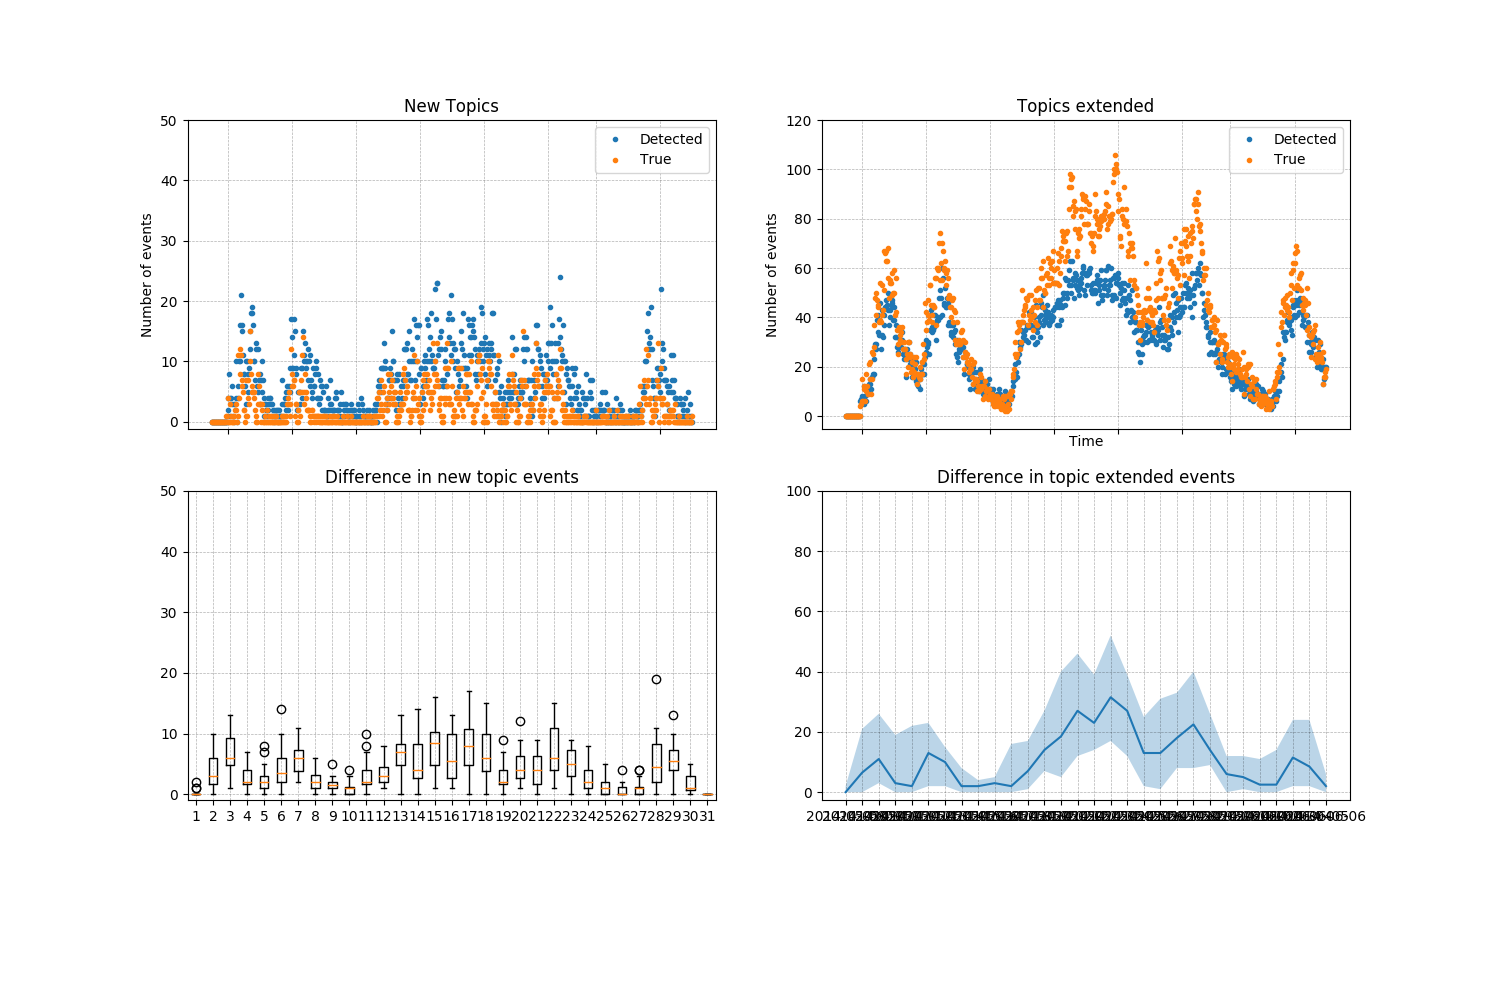
\includegraphics[width=1\textwidth]{event_detection_by_date_3000}
    \caption{Number of events with a batch size of 3000.}
    \label{fig:event_detection_by_date_3000}
\end{figure}

The raw data in \figref{fig:event_detection_by_date_3000}
also shows a direct correlation between the number of detected new events and the number of detected changes in events.
The more changes we missed, the more new events are detected.
This is to be expected,
since the detection of changes depends upon finding similar pairs of clusters in two different batches.
If a cluster in the current batch could not be matched to a cluster from the previous batch,
the cluster from the current batch will be seen as a new event.
Therefore the accuracy in finding pairs of clusters in crucial to a better performance.
The online clustering makes use of \gls{lsh} to find similar news articles
as explained in \subsubsecref{subsubsec:4c_implementation}.
The current threshold value for determining the similarity is set to 0.75.
To see the impact of the similarity threshold,
we run the online clustering again with a batch size of n=3000 and different thresholds.

\begin{figure}[h]
    \centering
    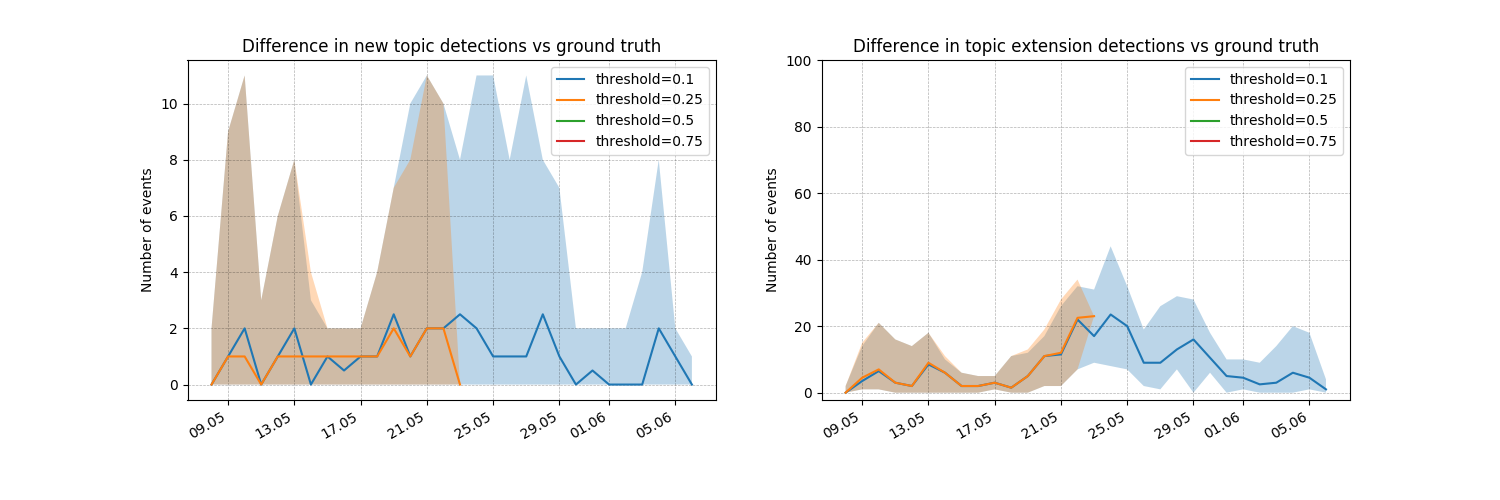
\includegraphics[width=1\textwidth]{event_detection_differences_threshold}
    \caption{Differences in detected over true events with different thresholds and a batch size of 3000.}
    \label{fig:event_detection_differences_threshold}
\end{figure}

\paragraph{Similarity threshold}
\figref{fig:event_detection_differences_threshold}
shows the effect of the threshold on the difference between detected and true events.
We see how the initial threshold of 0.75 was set too high,
as lower threshold such as 0.1 provide a considerably lower difference.
While there is still a substantial variance per day the median of the thresholds 0.1 and 0.5
is generally more stable and lower than with a threshold of 0.75.
The reason for the better performance of lower thresholds,
is that the overlap between batches decreases with an increase in the volume of news articles.
This is clearly visible during the peaks in \figref{fig:event_detection_differences_threshold}.
Thus a high similarity threshold cannot be met,
since there exists only an overlap of a few news articles for the same cluster between batches.
The MP-Score is also improved for new events as can be seen in \figref{fig:event_detection_mp_score_3000_0_1}.
While there is more variance than in similar plots from \figref{fig:event_detection_mp_score_1000}
and \figref{fig:event_detection_mp_score_5000},
the median from using threshold=0.1 clearly surpasses any measure from using threshold=0.75.
The high variance in the boxplot is due to the fact, that there are only a few new events per hour, if any.
This means detecting no events, when there are none leads to a score of 1,
while detecting one event, when there is none, leads to a score of 0.

\begin{figure}[h]
    \centering
    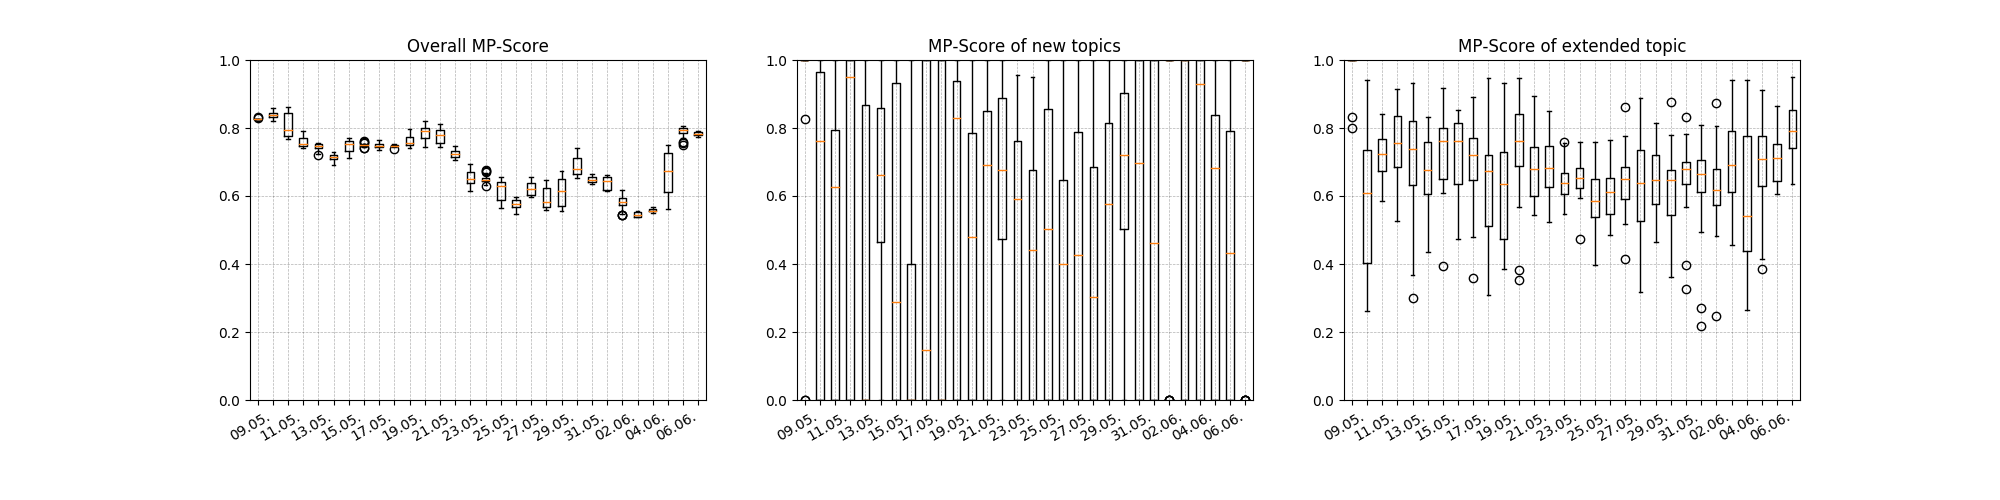
\includegraphics[width=1\textwidth]{event_detection_mp_score_3000_0_1}
    \caption{MP-Scores for online clustering with batch size n=3000 and threshold=0.1.}
    \label{fig:event_detection_mp_score_3000_0_1}
\end{figure}

\paragraph{Dynamic batch sizes}
After having analysed the impact of different batch sizes in detail and the similarity threshold,
we want to explore the result of using a dynamic batch size.
The first dynamic method loads the number of samples over $n$ hours.
The second dynamic method calculates the batch size based on the incoming samples and a predefined factor.
The dynamic methods will run with a similarity of 0.1 and an upper limit of 30,000 samples,
which is approximately 1,000 stories.
The number of the upper limit is based on observations from the clustering method evaluation.
Higher number of samples resulted in lower scores, while running into memory issues.

\figref{fig:event_detection_differences_hours} shows the difference in detected events
compared with the true number of events using the first dynamic method.
The variance is still quite high, especially during the peaks
where a lot of news articles are present in the data stream.
The best performance is achieved by setting the time window to 24 hours.
The average score for the overall clustering is 0.717 with a standard deviation of 0.119.
The detection of new events results in an average score of 0.618 with a standard deviation of 0.426
and the detection of changes results in an average score of 0.694 with a standard deviation of 0.16.
The resulting scores are better than with using a fixed batch size of 3,000, but not by much.
The biggest difference is in the average score of the detection of new events,
where this method is better by 0.076.
Increasing the time window to 48 or 72 hours results in slightly lower scores.

\begin{figure}[h]
    \centering
    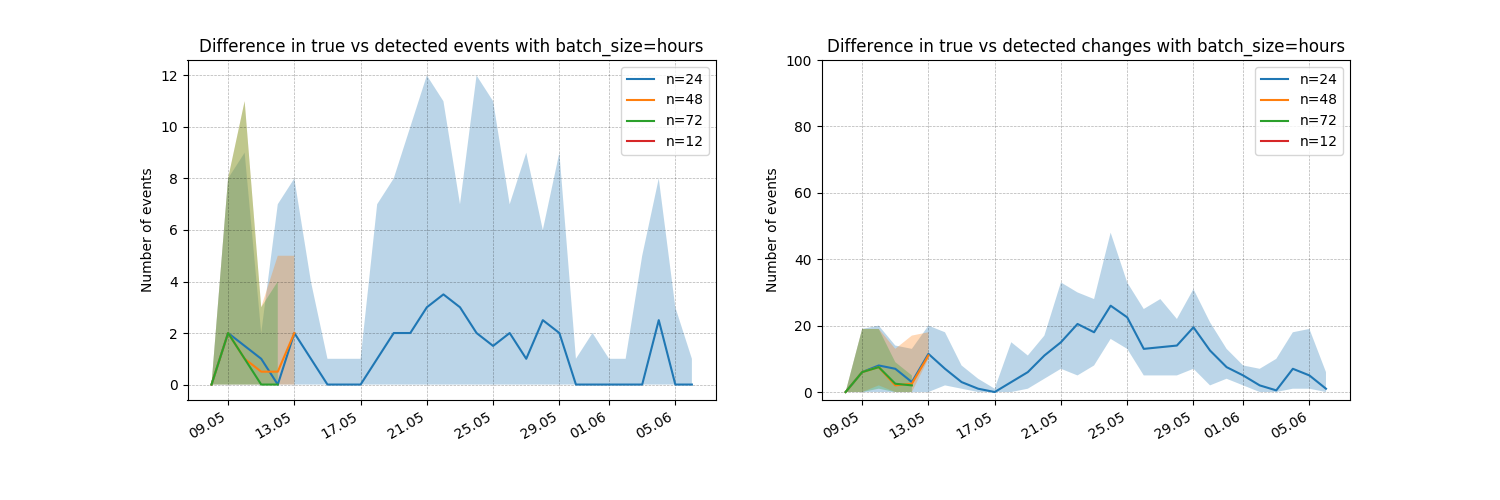
\includegraphics[width=1\textwidth]{event_detection_differences_hours}
    \caption{Difference in detected events vs predict events by using a dynamic batch size based on hours.}
    \label{fig:event_detection_differences_hours}
\end{figure}

Since the first dynamic method only showed a marginal improvement over the static method,
we move on to the second dynamic method.
In addition to an upper bound, this method uses a lower bound
to prevent the overlap between batches from becoming too small.
The lower bound is set to 3,000, since the evaluation of a fixed batch sizes proved 3,000 to provide the best results.
Our initial assumption was, that having a good lower bound
would give a good baseline and the relative factor allows the batch size
to grow with the increase in the volume of samples.
The overall performance should therefore be superior to using only the fixed batch size.
The data proved our assumption to be incorrect as can be seen in \figref{fig:event_detection_differences_hours}.
The best scores are achieved by using a factor of 25.
The overall score is 0.692 with a standard deviation of 0.091.
The detection of new events results in a score of 0.589 with a standard deviation of 0.429.
The score of detecting changes is 0.682 with a standard deviation of 0.136.

\begin{figure}[h]
   \centering
   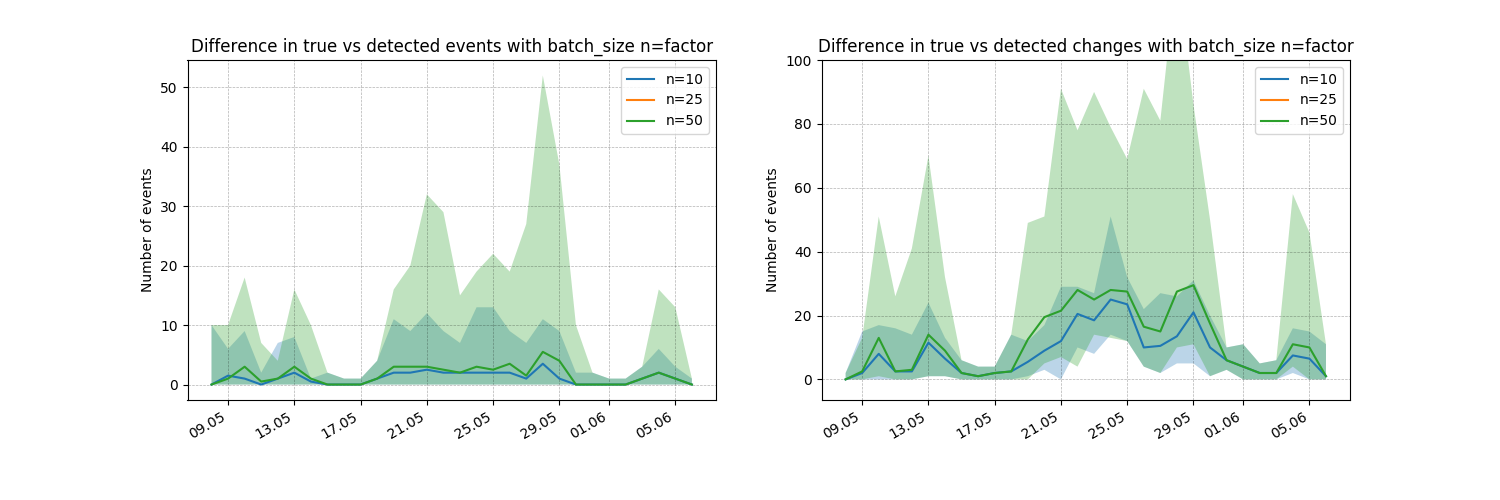
\includegraphics[width=1\textwidth]{event_detection_differences_relative}
   \caption{Difference in detected events vs predict events by using a dynamic batch size based on incoming samples.}
   \label{fig:event_detection_differences_relative}
\end{figure}

In addition, the data shows an interesting observation, where using a factor of 50 results in some extreme outliers.
The reason can be explained based on our previous clustering evaluation,
where we showed the decrease in precision with larger number of samples.
\figref{fig:nrows_by_new_rows} shows the maximum number of samples processed in a single batch.
The factor 50 reaches the upper limit during most peaks in the data stream.
Clustering with 30,000 resulted in an lower average score of roughly 0.24 compared to the best result.
Therefore an increasing amount of news articles is classified as noise and stories
are further fragmented into multiple clusters.
This leads to even bigger decreases in the event detection as this data shows.

\begin{figure}[h]
    \centering
    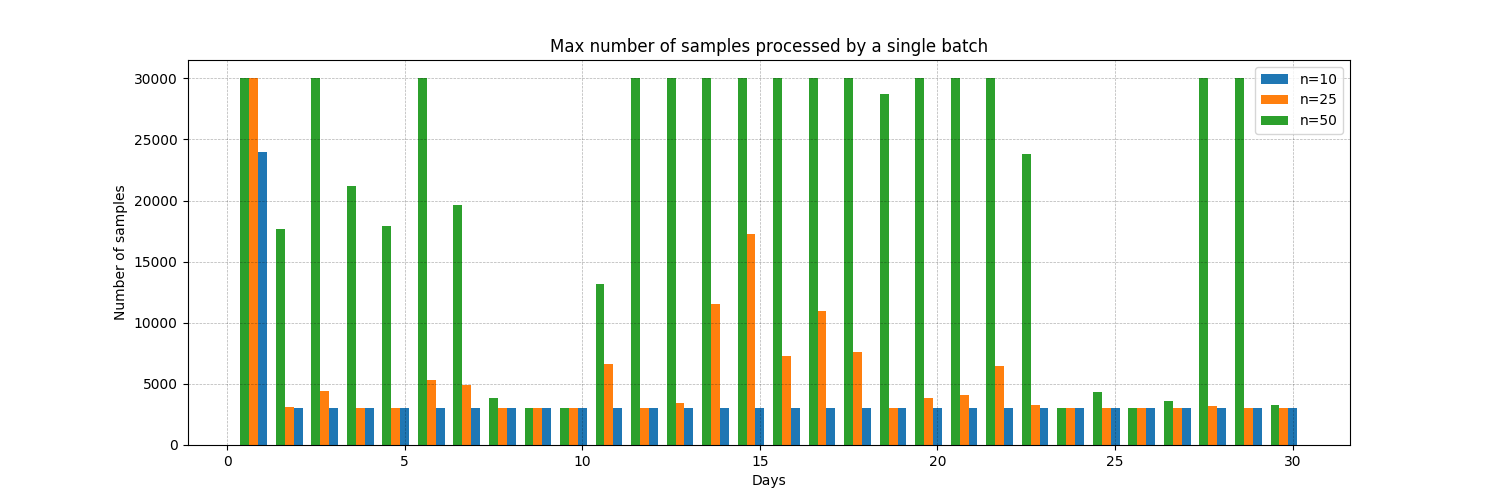
\includegraphics[width=1\textwidth]{nrows_by_new_rows}
    \caption{Maximum number of processed samples in a single batch per day and factor.}
    \label{fig:nrows_by_new_rows}
 \end{figure}

To conclude the evaluation of different methods for setting the batch size \tabref{tab:batch_size_methods}
shows the best approach per method.
The highest scores are highlighted as bold.
Based on this data, the time based method seems to provide the best results,
although the differences between the methods are minor.
The high standard deviation for the detection of new events shows
that the detection is quite unstable in its current form.
Improving the precision and the stability for the event detection
is therefore dependent on improving the overall clustering precision,
since the dynamic methods for determining the batch size only show limited impact.

\begin{table}[h]
    \centering
    \scalebox{0.75}{
    \begin{tabular}{|l|r|r|r|r|r|r|}
        \hline
        \textbf{Batch size method} & \multicolumn{2}{ |c| }{\textbf{Overall clustering}}  & \multicolumn{2}{ |c|}{\textbf{New events}}  & \multicolumn{2}{ |c| }{\textbf{Changes in existing events}} \\
        \hline
         & Mean & Standard deviation & Mean & Standard deviation & Mean & Standard deviation \\
        \hline
        Fixed with n=3000 & 0.701 & \textbf{0.085} & 0.542 & 0.435 & 0.683 & 0.144\\ \hline
        Time based with hours=24 & \textbf{0.717} & 0.119 & \textbf{0.618} & \textbf{0.426} & \textbf{0.694} & 0.16 \\ \hline
        Relative with factor=25 & 0.692 & 0.091 & 0.589 & 0.429 & 0.682 & \textbf{0.136} \\ \hline
    \end{tabular}
    }
    \caption{Final scores obtained by each method for setting the batch size.}
    \label{tab:batch_size_methods}
\end{table}

\paragraph{Noise rate}
One of the major factors in the lower precision of event detection
compared with the overall clustering is the noise rate.
To demonstrate this let us look at an online clustering over a simulated time period of five days.
Overall the time period includes 364 stories with 12,603 news articles.
During the online clustering we detected 275 new events and 4,080 changes.
On average these events contain 2 news articles.
Of the original 12,603 news articles only 8,626 have been assigned to clusters,
with an average cluster size of 26.4.
This results in a noise rate of 31.6\%.
If we now compare the average cluster size of 26.4 with the average event size of 2,
we can see how single events are more likely to be missed than clusters due to their size.

During the analysis we also looked at two specific examples "Gmail redesign" and "Bad Neighbours".
The first example was detected without errors,
while the second example contained multiple news articles discarded as noise and a fragmentation in clusters.
The fragmentation means that news articles from the same story got assigned to different clusters during the same batch,
resulting in incorrect events.

The difference in the performance of both examples, can be explained based on the contents of their news articles.
The first example about the "Gmail redesign" consists mostly of technology focused news sites
such as \textit{Ars Technica} or \textit{PC Magazine}.
Therefore the contents of the news articles are of good quality and share the same technical vocabulary.
The second example with the new release of the film "Bad Neighbours"
has a wider variety of sources and types of articles.
Some news articles are short summaries, while others are interviews or personal reviews.
As a result the vocabulary is more general than compared to the technical articles and varies stronger between articles.
This leads to increased differences in the tf-idf model,
which we have already explored as part of the clustering evaluation.

\subsubsection{Conclusion}
\label{subsubsec:5b_conclusion}

We explored different methods for determining the batch size, with one static and two dynamic approaches.
The best results were achieved by using the dynamic method,
which loads samples from the last 24 hours instead of defining an actual batch size.
The resulting precision of the clustering using this method is 72\% with a standard deviation of 12\%.
The precision for detecting new events results in 62\% with a standard deviation of 43\%.
Detecting changes in existing events results in a precision 69\% with a standard deviation of 16\%.
Although the differences in the resulting scores between the methods are marginal
and all methods show similar deviations in the event detection.
One of the reasons the dynamic methods did not perform better,
is based on the overall decrease in precision of HDBSCAN with higher number of samples.
Therefore increasing the batch size to react to high volumes of traffic
resulted in a score similar or worse than the static batch size.
In addition, we compared different thresholds for defining the similarity between samples
and found 0.1 to be a good candidate.
The noise rate is shown to impact the events even more then the clusters
and therefore is a major influence regarding the precision of the event detection.
In conclusion the high variance in correctly detecting event shows,
that it is quite unstable in its current form and further optimizations should be focused
on the overall clustering and on lowering the noise rate.
